\begin{figure}[t]
  \centering
  \begin{subfigure}[t]{0.48\textwidth}
    \centering
    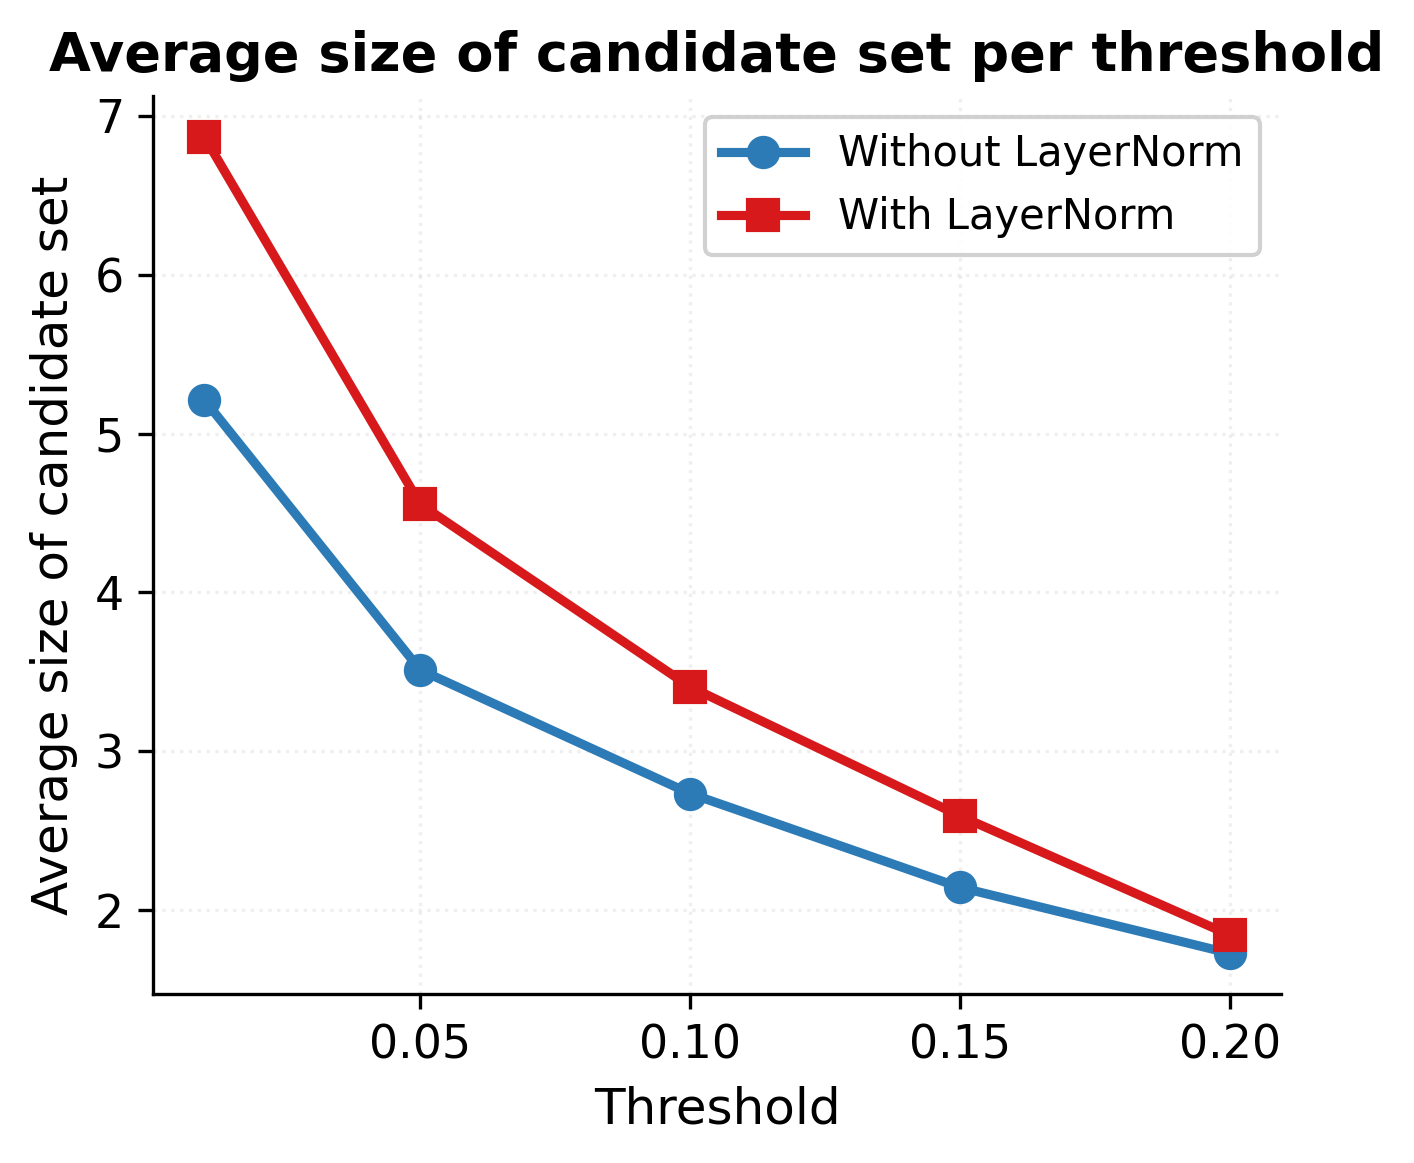
\includegraphics[width=\linewidth]{results/topk_and_candidateset/count_comparison.png}
    \label{fig:candidate_set_size}
  \end{subfigure}
  \hfill
  \begin{subfigure}[t]{0.48\textwidth}
    \centering
    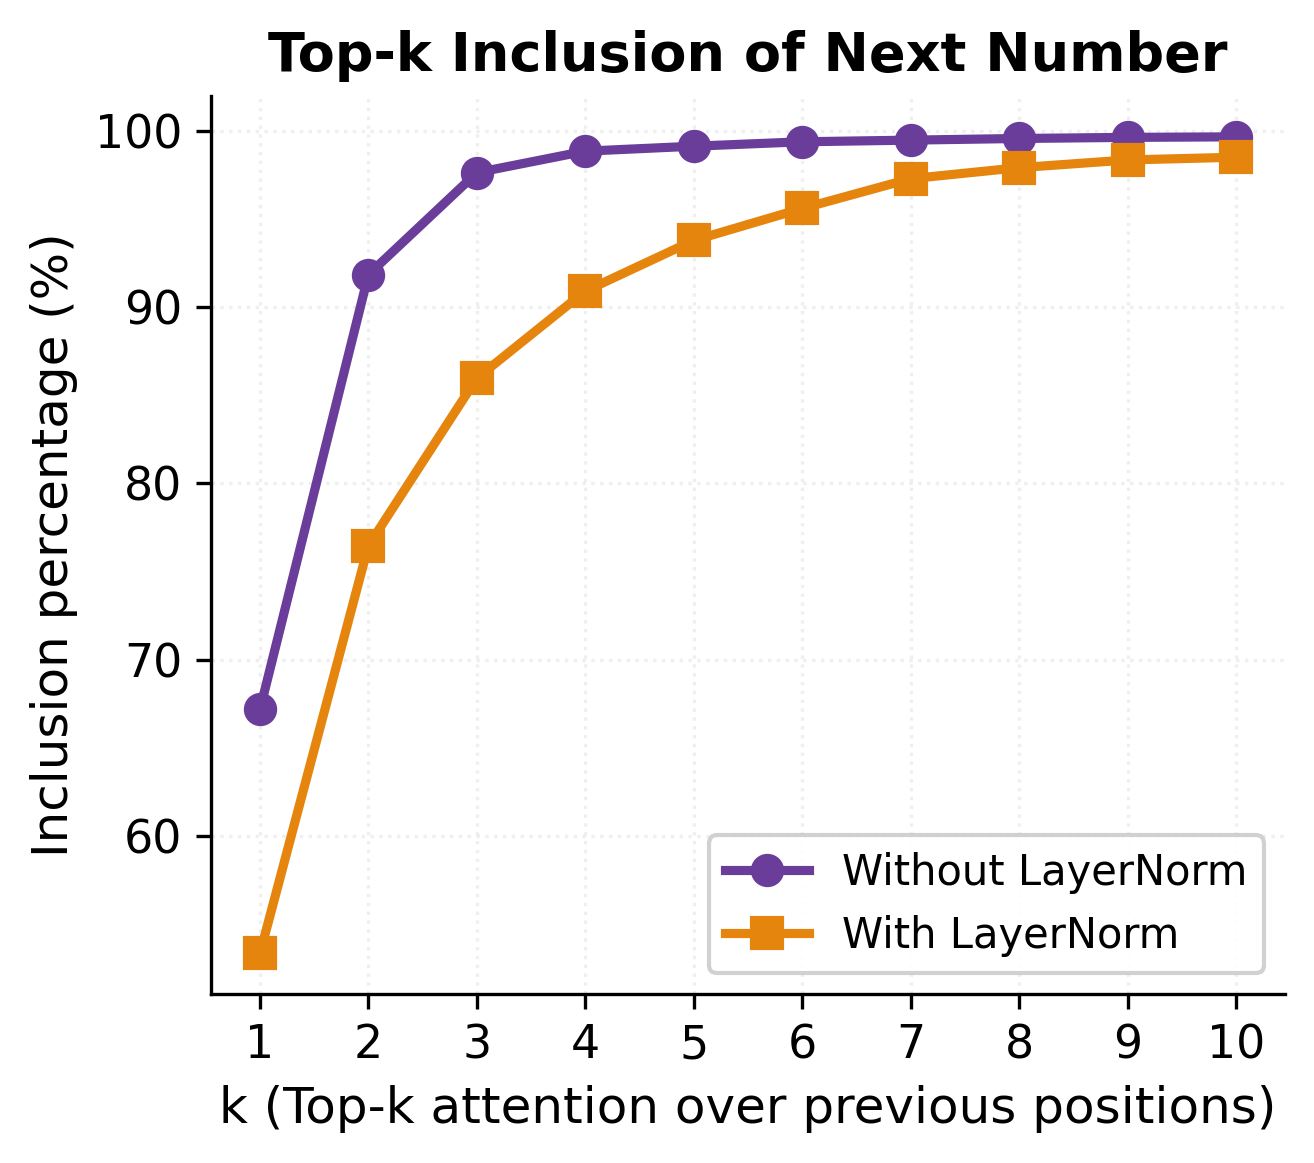
\includegraphics[width=\linewidth]{results/topk_and_candidateset/compare_topk_inclusion.png}
    \label{fig:topk_inclusion}
  \end{subfigure}
  \caption{Comparison of attention-based retrieval between models trained with and without layer normalization. \textbf{(Left)}~Average size of the candidate set (tokens whose attention score exceeds a given threshold) as a function of the threshold. \textbf{(Right)}~Percentage of decoding positions at which the correct next token appears among the top-$k$ attended previous positions, as a function of~$k$. Both models achieve near-perfect inclusion by $k{=}5$, indicating that the first attention layer reliably assigns high scores to the token that should be produced next.}
  \label{fig:topk_and_candidateset}
\end{figure}
